% Generated by scripts/report_figures.py; data inline.
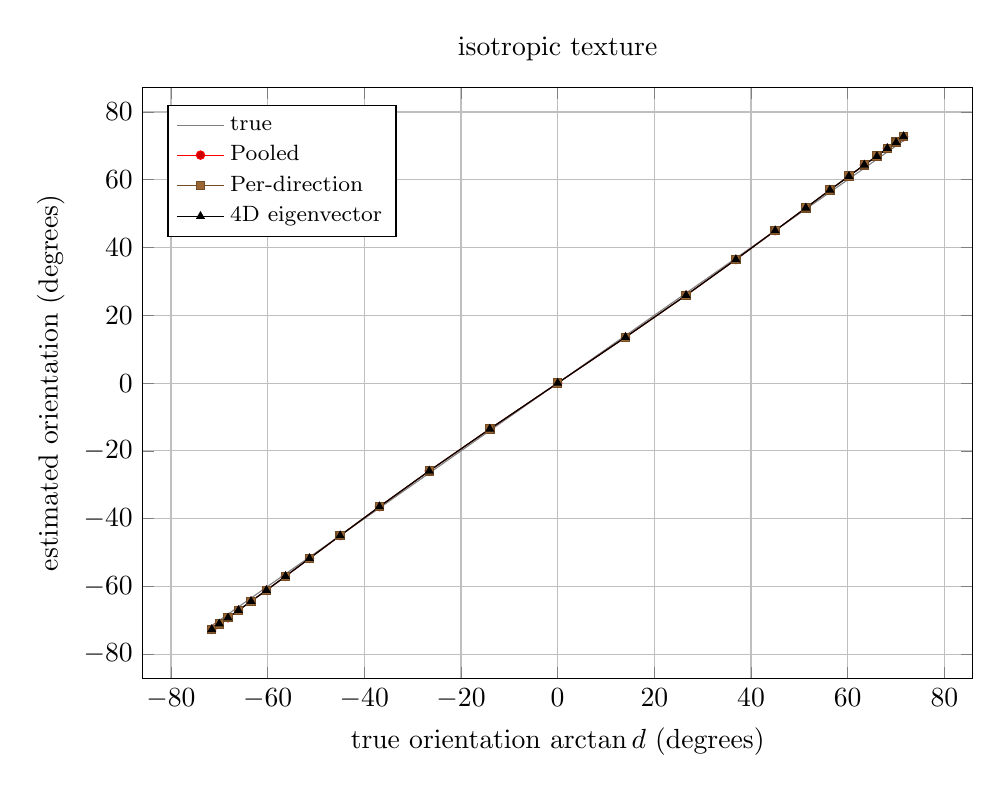
\begin{tikzpicture}
\begin{axis}[width=\linewidth, height=0.75\linewidth, xlabel={true orientation $\arctan d$ (degrees)}, ylabel={estimated orientation (degrees)}, grid=major, legend pos=north west, legend cell align=left, legend style={font=\footnotesize}, title={isotropic texture}]
\addplot[gray, thin, domain=-71.5651:71.5651] {x};
\addlegendentry{true}
\addplot+[mark=*, mark size=1.5pt] coordinates {(-71.5651,-72.676) (-70.0169,-71.0861) (-68.1986,-69.2496) (-66.0375,-67.0413) (-63.4349,-64.3696) (-60.2551,-61.1677) (-56.3099,-57.0303) (-51.3402,-51.7423) (-45,-45.0001) (-36.8699,-36.451) (-26.5651,-25.9027) (-14.0362,-13.522) (0,-0.000180645) (14.0362,13.5205) (26.5651,25.9097) (36.8699,36.4542) (45,44.9994) (51.3402,51.7164) (56.3099,56.9862) (60.2551,61.0875) (63.4349,64.3909) (66.0375,67.0253) (68.1986,69.2584) (70.0169,71.1065) (71.5651,72.7141)};
\addlegendentry{Pooled}
\addplot+[mark=square*, mark size=1.5pt] coordinates {(-71.5651,-72.6748) (-70.0169,-71.0861) (-68.1986,-69.2507) (-66.0375,-67.0401) (-63.4349,-64.3722) (-60.2551,-61.1674) (-56.3099,-57.0292) (-51.3402,-51.743) (-45,-45.0001) (-36.8699,-36.4509) (-26.5651,-25.9026) (-14.0362,-13.5215) (0,-0.000163267) (14.0362,13.5203) (26.5651,25.9097) (36.8699,36.4545) (45,44.9994) (51.3402,51.7164) (56.3099,56.9867) (60.2551,61.0872) (63.4349,64.3909) (66.0375,67.0268) (68.1986,69.2563) (70.0169,71.1069) (71.5651,72.7141)};
\addlegendentry{Per-direction}
\addplot+[mark=triangle*, mark size=1.5pt] coordinates {(-71.5651,-72.6795) (-70.0169,-71.0238) (-68.1986,-69.2443) (-66.0375,-67.0504) (-63.4349,-64.3882) (-60.2551,-61.1182) (-56.3099,-57.0018) (-51.3402,-51.7235) (-45,-44.9989) (-36.8699,-36.4528) (-26.5651,-25.9166) (-14.0362,-13.5331) (0,0.00128684) (14.0362,13.5469) (26.5651,25.9242) (36.8699,36.4699) (45,44.9992) (51.3402,51.702) (56.3099,56.978) (60.2551,61.0615) (63.4349,64.3884) (66.0375,66.9292) (68.1986,69.2768) (70.0169,70.9866) (71.5651,72.7863)};
\addlegendentry{4D eigenvector}
\end{axis}
\end{tikzpicture}
